\documentclass[11pt]{article}

\usepackage[margin=1in]{geometry}
\usepackage{amsmath, amssymb}
\usepackage{hyperref}
\usepackage{enumitem}
\usepackage{booktabs}
\usepackage{tikz}
\usetikzlibrary{arrows.meta, positioning}

\title{Structural Reliability Under Projection:\\
Representational Loss, Reconstructibility, and Admissibility}

\author{Brian Cameron}
\date{August 15, 2026}

\begin{document}

\maketitle

\begin{abstract}
AI systems increasingly reason and act from compressed representations: prompts, summaries, retrieved passages, logs, metrics, traces, memory, and policy artifacts. Such representations may collapse distinctions required by downstream claims while leaving those claims locally coherent. This paper characterizes that failure as query-relative representational loss rather than ordinary inference error. For a projection \(P:S\rightarrow R\), a query is identifiable only when states collapsed by \(P\) do not require different answers. When that condition fails, additional reasoning over \(R\) cannot universally recover the missing distinction.

The paper develops a dependency-status account---preserved, reconstructible, traceable, and opaque---that links represented support to licensed answer form, while separating informational support from operational permission. It further distinguishes actual, assessed, and reported dependency status and identifies a second-order limit on self-certifying admissibility procedures.

The objective is not perfect reasoning or complete representation. It is diagnostic legibility: preserving enough structure that materially relevant uncertainty, loss, assumptions, and unsupported dependencies can be exposed rather than silently promoted into determinate claims. Representations may be revised as inquiry reveals new dependencies, but such refinement should respond to demonstrated diagnostic need rather than an aspiration to encode all potentially relevant state. The framework therefore treats reliability under projection as the disciplined management of visible and correctable failure.
\end{abstract}

\section{Introduction: Local Coherence Without Structural Admissibility}

This paper is intended as a conceptual bridge between formal accounts of identifiability and practical concerns in AI reasoning, safety, security, and agentic reliability. Its central claim is that many AI reasoning failures are not simply wrong inferences, but unsupported inferences from representations that do not preserve the distinctions required by the query. This matters for systems that answer from prompts, summaries, retrieval results, logs, traces, metrics, policy artifacts, or compressed context windows: the system may produce a locally coherent answer while the representation itself does not support the conclusion.

The novelty claimed here is not that projection can destroy identifiability, sufficiency, or task-relevant information. Those phenomena are well established in statistics, decision theory, abstraction, partial-observation models, and information theory. The additional step taken here is operational: the framework treats the relation between a claim and its represented support as a licensing relation that constrains the epistemic form in which a reasoning system may answer.

Accordingly, the framework asks not only whether a query remains identifiable, but what a bounded reasoner may responsibly claim when the operative representation preserves the required distinction directly, makes it boundedly reconstructible, leaves it merely traceable, or does not preserve an auditable dependency at all. It further distinguishes the dependency status that actually obtains from the status a bounded reasoner assesses and the status it ultimately reports. The distinctive progression is therefore
\[
\boxed{
\text{projection}
\rightarrow
\text{dependency status}
\rightarrow
\text{licensed response form}
\rightarrow
\text{reported epistemic status}.
}
\]

This licensing relation has two conceptually distinct aspects. The first is query-relative support: whether the representation preserves or boundedly reconstructs the distinctions required by the claim. The second is operational validity: whether a proposed action or continuation is permitted within the declared regime, or can be returned to that valid region by bounded correction. An answer may be informationally supported while the action it proposes remains operationally invalid.

As a running example, consider an AI assistant used during a security incident. It receives a compressed summary of logs, deployment history, alerts, and recent configuration changes. The assistant produces a clear root-cause explanation and recommends a fix. The reasoning may appear locally coherent: it cites the deployment, explains the failure, and proposes remediation. However, the compressed representation may not preserve the distinction between a deploy-triggered bug, a dependency outage, a configuration interaction, and telemetry loss caused by reduced logging. If the available representation cannot distinguish these states, then the assistant has not merely made an error. It has produced a determinate explanation from a representation that does not support one. Even if the assistant could support a diagnostic claim, the proposed fix would require a separate operational judgment: whether the intervention is authorized, reversible, locally bounded, and valid under the current incident regime. Informational support for the diagnosis does not by itself license the action.

The corrective objective in such a case is not to anticipate and represent every variable that might ever matter to an incident. Suppose instead that successive incidents repeatedly end with several causes remaining indistinguishable because event ordering, logging state, or a particular configuration relation was not retained. That recurring diagnostic failure is evidence that the operative representation is insufficient along a demonstrated dimension. The appropriate refinement may be additional telemetry, provenance, retained event ordering, or a targeted diagnostic probe rather than general expansion of the system's ontology. In this sense, representational structure should be refined under diagnostic pressure: a distinction earns continued representation when observed failures, ambiguities, or unresolved alternatives demonstrate that its absence materially limits diagnosis or correction.

A further reason to privilege diagnostic legibility is that consequential failure classes cannot always be specified in advance. This is especially clear in security and other adversarial or open-ended domains, where a novel failure may exploit a dependency, interaction, or abstraction boundary that the original system model did not recognize as material. Structural reliability should therefore not be understood only as detecting a predefined catalogue of errors or losses. A representation should, where practical, preserve enough attributable structure that unexpected mismatch can motivate the discovery of a new distinction, dependency, or failure class. Diagnosability is in this sense prospective: the system should support learning what kind of failure occurred even when that category was not fully represented before the failure.

More generally, the problem can be understood as one of invariant preservation under projection. A claim remains admissible only when the distinctions on which it depends are preserved, boundedly reconstructible, or explicitly marked as unavailable. Projection is dangerous not because it compresses, but because it can collapse the invariants required by a downstream claim while leaving the answer form unchanged. Good reasoning under projection therefore requires preserving the dependency structure needed by the claim, or changing the response form when that structure no longer survives.

A loss-relevant dependency need not determine the factual answer directly. A projection may preserve every distinction required to recover a factual endpoint while erasing structure required to determine how the surviving information is permitted to participate in downstream reasoning. Factual sufficiency and governance sufficiency may therefore diverge while remaining instances of the same query-relative projection problem.

The dependency structure required by a query should not be understood as fixed, complete, or necessarily known before reasoning begins. Practical inquiry may reveal that the original question collapsed several questions, that a familiar term has incompatible meanings, that an action requires a separate authority or validity judgment, or that an existing concern bears upon a claim not previously associated with it. The present framework therefore applies to the dependencies currently represented as material to the query, while allowing that later inquiry may revise that structure.

In AI safety and security settings, the dangerous failure is often not that a model is uncertain. It is that the model behaves as though a missing distinction were recoverable from the representation available to it. This can occur when a security assistant recommends a fix without the relevant code path or threat model, when a RAG system treats a citation pointer as source support, when an incident-response assistant names a root cause despite indistinguishable telemetry, or when an agent acts as if authorization, intent, or environmental state were known from compressed memory. These issues connect to broader concerns about robustness and failure modes in AI systems~\cite{Amodei2016}.

These failures share the same structural form: the response presents a stronger dependency status than the operative representation supports.

A related failure can occur when projection preserves a useful reasoning operation while collapsing the conditions that governed its use. A heuristic, diagnostic procedure, review pattern, reasoning scaffold, or inherited decision rule may remain executable after its originating assumptions, scope restrictions, corrective mechanisms, provenance, or authority conditions are no longer represented. The operation may therefore continue to produce locally coherent, and sometimes even correct, results even when the current representation no longer supports the judgment that applying it is appropriate. Preserving an operation is not equivalent to preserving the conditions governing its application.

The account is normative in a limited epistemic sense. It does not describe how reasoning systems always behave or prescribe substantive decisions or values. It proposes admissibility criteria for reasoning under compression: a system should not present a conclusion as determined by a representation when the relevant query depends on a distinction that the representation does not preserve, cannot boundedly reconstruct, and cannot justify without changing the information basis or answer form. Admissibility is therefore query-relative. A projection is not defective merely because it compresses; it becomes inadmissible for a particular use when the downstream claim depends on a collapsed distinction.

The resulting evaluation question is therefore directly relevant to AI reasoning, safety, and security evaluation. It asks whether a system can distinguish supported inference from decision under non-identifiability; whether it can mark when source support is traceable but not reconstructible; whether it can avoid collapsing system-level failures into single actors; and whether it can keep correction bounded to the information actually available. These conditions matter because safety failures often occur at the boundary between what the system can infer, what it must assume, and what it should route, defer, or refuse.

This paper contributes a structural account of reliability under projection organized around six ideas. First, it distinguishes correctable error from query-relative representational loss. Second, it identifies a task-relative exact-sufficiency baseline against which projected representations can be understood. Third, it distinguishes loss introduced in forming the reasoning target from loss introduced when that target is subsequently represented. Fourth, it classifies dependencies both by structural role and by support status---preserved, reconstructible, traceable, or opaque. Fifth, it distinguishes actual dependency status from the status assessed and reported by a bounded reasoner, yielding a second-order limit on self-certifying admissibility procedures. Sixth, it argues that response form must weaken when dependency support weakens or when operational validity cannot be established or boundedly restored. Together these claims treat answer form as part of reasoning validity rather than merely a stylistic choice.

\section{Reasoning Under Projection}

To understand these failures, we must examine the conditions under which reasoning operates. In practice, reasoning systems do not operate on complete representations of the problems they address.

\subsection{Reasoning Over Representations}

Any reasoning process operates on a representation of the problem rather than the full underlying system. In AI systems, that representation may be a prompt, retrieved context, tool output, memory state, log summary, embedding, schema, score, or policy artifact. The question is not whether the representation is complete; it is whether it preserves the distinctions required by the claim being made.

\paragraph{Operative representation in LLM systems.}
For language models, the operative representation is not simply the user prompt. It includes the information basis available to the model for the current answer: the prompt, conversation state, retrieved passages, tool outputs, exposed memory, structured metadata, policy constraints, explicit assumptions, uncertainty markers, and any prior or background knowledge that the system is permitted to rely on for the task. This boundary is often fuzzy. The framework does not require that all internal model state be inspectable. It requires that claims be calibrated to the support that is available, exposed, or explicitly invoked in the answer. If a claim depends on latent background knowledge, an unavailable source, a hidden prior, or a tool result not present in the answer context, then that dependency should be marked rather than presented as if it were determined by the visible representation alone.

For licensing purposes, it is useful to preserve the roles played by different parts of this information basis rather than collapsing them into an undifferentiated \(R\). Where the distinction is material, write schematically

\[
R
=
\langle
R_E,\,
R_B,\,
R_D
\rangle,
\]

where \(R_E\) denotes represented evidence or observations, \(R_B\) denotes explicitly invoked background knowledge, priors, assumptions, or model commitments, and \(R_D\) denotes decision-relevant policy, utility, authority, or operational constraints. This notation is a typed view of the operative representation, not an assumption that the components are independent or implemented as separate stores.

The distinction matters because support should retain its basis. A conclusion may be underdetermined by \(R_E\) while being preferred under an explicit prior in \(R_B\), and an action may be selected under a policy in \(R_D\) without thereby becoming evidentially determined by \(R_E\). Thus,

\[
\boxed{
\text{evidence-supported}
\neq
\text{prior- or assumption-supported}
\neq
\text{policy-selected}.
}
\]

Treating all three as merely ``represented'' would preserve their presence while collapsing the epistemic role each one actually plays.

The same principle applies within provenance and source use. Preserving a source and its factual content does not necessarily preserve the role that source was permitted to play. Information may, for example, be permitted to support a hypothesis, challenge a conclusion, or trigger verification without being permitted to select an operational parameter directly. Such role distinctions are themselves dependencies that projection may preserve, collapse, or erase.

\subsection{Projection as Compression}

We define \emph{projection} as any transformation that maps a richer system state into a reduced representation used for reasoning. Projection may be lossy in the information-theoretic sense~\cite{Shannon1948}, but the relevant issue for reasoning is whether the reduced representation preserves the distinctions required for later inference, decision, or evaluation. Equivalently, the concern is not compression as such, but whether the projection discards task-relevant sufficient information for the query being asked.

Formally, projection can be understood as a mapping:
\[
P: S \rightarrow R
\]
where $S$ is the full system state and $R$ is the representation used for reasoning.

In many AI settings, \(S\) should be understood as a modeled or idealized underlying state space rather than a fully specified object available to the system. The framework is therefore relative to the state model under consideration.

\subsection{Target Formation and Representational Projection}

The mapping \(P:S\rightarrow R\) begins from a state space \(S\) already treated as the target of reasoning. Swanson distinguishes an upstream boundary operation that stabilizes a target from a subsequent rendering operation that produces a finite representation of that target~\cite{Swanson2026Monist}. Adapting that distinction to the present notation, a richer account may therefore distinguish target formation from subsequent projection:

\[
F \xrightarrow{B_{\Gamma}} S_{\Gamma}
  \xrightarrow{P_{\Gamma}} R,
\]

where \(F\) denotes a broader field of potentially relevant state, \(B_{\Gamma}\) selects or constructs the state space treated as relevant under regime \(\Gamma\), and \(P_{\Gamma}\) maps that selected state into the operative representation.

This distinction separates two structurally different sources of insufficiency. \emph{Target-selection loss} occurs when \(B_{\Gamma}\) excludes a distinction that is material to the downstream query. \emph{Representational loss} occurs when the selected state \(S_{\Gamma}\) contains the relevant distinction but \(P_{\Gamma}\) fails to preserve or boundedly reconstruct it in \(R\). The simpler notation \(P:S\rightarrow R\) used throughout this paper should therefore be understood as conditioning on a currently declared target state \(S\); it does not imply that the construction of \(S\) was itself lossless or complete.

The distinction matters operationally because representation repair and target revision are not the same intervention. Enriching \(R\) may repair a lossy projection from \(S_{\Gamma}\) while leaving untouched a material distinction that was excluded when \(S_{\Gamma}\) was formed. Conversely, revising the target boundary may reveal that a previously adequate projection was answering the wrong or incomplete question.

Multiple distinct states in $S$ may map to the same representation in $R$.

In information-theoretic terms, $R$ can be treated as the information basis available to the reasoner after projection. The relevant question is not whether $R$ contains less information than $S$ in general, but whether it retains the information needed to answer the query at hand. A representation may be highly compressed and still sufficient for one query, while being insufficient for another query that depends on a collapsed distinction.

A simple example illustrates the query-relative nature of projection. A black-and-white image may preserve shape while losing color. It remains admissible for many shape queries, but not for a query that depends on whether an object was red or green. The projection is not defective in general; it is insufficient for queries whose answers depend on the collapsed distinction.

Projection may likewise preserve procedures rather than only observable features. A compressed representation may retain a rule such as “when condition x appears, apply operation f” while omitting distinctions that originally limited when f was appropriate. The procedure therefore remains executable even though the query “is f licensed in this case?” may no longer be identifiable from the compressed representation. This is an important form of representational loss because operational continuity can conceal contextual loss: the persistence of a usable transformation may create the appearance that the conditions supporting that transformation were preserved as well.

Equivalently, projection determines which distinctions remain observable through the representation. This observable distinction structure can be formalized using the language of representation-induced $\sigma$-algebras: a query is directly supported only when the distinction it requires is measurable under the projected representation, or becomes available through bounded reconstruction.

In this paper, projection refers specifically to transformations that induce non-trivial equivalence classes over the underlying state space: distinct states in $S$ are mapped to the same representation in $R$.

The analysis is relative to a given projection $P$. A query may fail to be identifiable under one representation while becoming identifiable under a richer or differently structured representation. For example, a log summary may preserve that an outage occurred while losing the event ordering needed for root-cause analysis. A retrieval result may preserve a citation identifier while omitting the source passage needed to verify the claim. A risk score may preserve a ranking while losing the distinction between reversible and irreversible failures. These projections are useful, but they are not equally admissible for every downstream query.

In practice, however, reasoning systems often operate under fixed or externally imposed projections: a prompt, summary, metric, ranking, category, analogy, translation, dataset schema, interface boundary, token budget, or institutional decision format may determine what information is available at inference time. The question addressed here is therefore not whether some better representation could exist, but what follows when reasoning must proceed under the representation actually available.

\subsection{Equivalence Classes and Collapse of Distinction}

Because projection is many-to-one, it induces equivalence classes over the original state space. Distinct underlying states become indistinguishable once projected into the representation.

This means that some distinctions present in the original system may no longer be available to the reasoning process through the current representation. For the query being asked, those distinctions are not merely hidden within the representation; they are unavailable unless additional assumptions, structure, or observations are introduced.

This is the point at which ordinary partial observability and representational loss diverge. In a partial-observation setting, the system may maintain a belief state over hidden possibilities still represented by the model. Under projection-induced loss, the distinction required by the query may not be represented in the current state space at all. No update over the current representation can recover such a distinction unless the representation is expanded, a bounded reconstruction path is available, or an explicit assumption is introduced and marked.

\subsection{Identifiability Under Projection}

Let $P:S\rightarrow R$ be a projection from system states to representations. The projection induces an equivalence relation on $S$:

\[
s_1 \sim_P s_2 \quad \text{iff} \quad P(s_1)=P(s_2).
\]

A query, judgment, or decision-relevant property $q:S\rightarrow A$ is identifiable under $P$ when it is constant over the equivalence classes induced by $P$:

\[
P(s_1)=P(s_2) \Rightarrow q(s_1)=q(s_2).
\]

For normative or evaluative queries, \(q\) should be read as model-relative: the framework analyzes whether a declared evaluative target is preserved under projection, not whether the target has a mind-independent unique value.

The use of identifiability here generalizes the term beyond parameter recovery in statistical or causal models. In this paper, identifiability refers to whether any reasoning-relevant query, judgment, or decision property survives projection into the representation used by the system.

If this condition holds, then the representation preserves enough information to answer $q$. If the condition fails, then two states that are indistinguishable in the representation require different answers to $q$. In that case, no reasoning process operating only on $R$ can determine $q$ without introducing additional assumptions, expanding the representation, or obtaining new information.

This gives a compact way to state the error--loss distinction. In the measure-theoretic formulation developed later, this corresponds to whether the query is measurable with respect to the observable structure induced by the projection. An error occurs when $q$ is identifiable under the projection but the reasoning process returns the wrong value. Loss occurs when $q$ is not identifiable under the projection, so the representation itself no longer supports a determinate answer.

In more familiar statistical and information-theoretic terms, error is a recoverable inference or estimation failure within an information basis that is sufficient for the query. Loss is a failure of sufficiency: the projection has discarded task-relevant information needed to distinguish states with different values of $q$. Equivalently, the projected representation is not a query-relative sufficient statistic for $q$.

\paragraph{Minimal example.}
Let \(S=\{s_1,s_2\}\), with \(P(s_1)=P(s_2)=r\) but \(q(s_1)\neq q(s_2)\). The same representation therefore corresponds to two different required answers, so \(q\) is not identifiable under \(P\).

\paragraph{Basic consequence: non-identifiability blocks recovery from the projected representation alone.}
If a query $q:S\rightarrow A$ is not identifiable under projection $P:S\rightarrow R$, then no function $f:R\rightarrow A$ can recover $q$ for all states in $S$.

This is an elementary consequence of the definition of a function, included only to make explicit the boundary between recoverable error and representational loss.

\emph{Argument.}
If $q$ is not identifiable, then there exist $s_1,s_2\in S$ such that $P(s_1)=P(s_2)=r$ but $q(s_1)\neq q(s_2)$. Any function $f$ over $R$ must assign a single value to $r$, so it cannot equal both $q(s_1)$ and $q(s_2)$. Therefore, any determinate answer requires an additional assumption, representation expansion, or information outside $R$.

\paragraph{Task-relative exact support.}
The identifiability condition also induces a canonical task-relative quotient of the underlying state space. This construction is closely related to Bruhacs's task-sufficiency and minimal-support treatment of reasoning under projection~\cite{Bruhacs2026Projection}. For the single query \(q:S\rightarrow A\), define

\[
s_1\sim_q s_2
\quad\text{iff}\quad
q(s_1)=q(s_2),
\]

and let

\[
Q_q=S/{\sim_q}.
\]

The quotient \(Q_q\) retains exactly the distinctions required to determine \(q\): states may be collapsed whenever they require the same answer, but not when they require different answers. Any representation sufficient to determine \(q\) must therefore distinguish at least the equivalence classes relevant to \(Q_q\), although it may encode those distinctions in a different form.

This provides a useful exact-sufficiency baseline for reasoning under projection. If the operative representation \(R\) preserves enough structure to distinguish the relevant classes of \(Q_q\), then the query is identifiable in principle. The primary concern of the present framework is the harder regime in which the operative representation falls below that task-relative threshold, or in which the reasoner cannot establish that the threshold has been met. The question then changes from ``what is the exact answer?'' to ``what response form remains licensed by the support that actually survives?''

\paragraph{Representation-or-form requirement.}
When a query is not identifiable under the current representation, an admissible response must either change the information basis or change the answer form. It may expand the representation, obtain new information, introduce an explicit assumption or decision rule, weaken the claim, branch over alternatives, mark the dependency as traceable, route the query, or refuse the requested form. What it must not do is present the unsupported determinate answer as if it followed from the original representation alone.

The formal claim is limited: non-identifiability means that no function over the current representation can recover the query for all underlying states. The design question is what a reasoning system should do when this condition holds. The remaining sections describe structural requirements and behavioral consequences, rather than additional formal impossibility results.

This separates the descriptive and normative parts of the argument. The descriptive claim is that non-identifiability prevents recovery of $q$ from $R$ alone. The normative claim is an epistemic admissibility criterion: a reasoning system should not present a conclusion as determined by $R$ when the conclusion depends on distinctions that $R$ does not preserve or make reconstructible. This criterion does not require inaction. It requires that action under non-identifiability be marked as a decision rule, assumption, conditional response, request for representation expansion, or unresolved dependency rather than as an inference licensed by the current representation. Non-identifiability does not imply silence; it changes the epistemic status of speech. For brevity, I refer to these moves---representation expansion, external information, explicit assumptions, conditionalization, routing, or refusal of the requested form---as changing the information basis or answer form.

Admissibility is intentionally weaker than correctness. The framework does not determine which decision procedure a system must use when $R$ is insufficient, nor does it prohibit probabilities, confidence intervals, ranked hypotheses, priors, utility functions, or policy choices. It constrains the epistemic status of the output: a claim should not be presented as following from $R$ alone when it depends on distinctions that $R$ does not preserve or make reconstructible. A probabilistic or decision-theoretic response may be admissible if it marks the assumptions, priors, utilities, or decision rules on which it depends; it becomes inadmissible when those elements are presented as if they were determined by the representation itself. This is especially important for AI safety and security because many unsafe outputs are not unsupported in the sense of being nonsensical; they are unsupported in the narrower sense that they present assumptions, priors, tool traces, or policy choices as if they were determined by the available evidence.

\paragraph{Immediate consequences.}
This observation yields three immediate consequences for reasoning under projection.

\emph{Unsupported determinacy.}
If $q$ is not identifiable under $P$, then any determinate answer to $q$ from $R$ alone must depend on assumptions not contained in $R$.

\emph{Correction boundary.}
If a failure concerns an identifiable query, correction can in principle operate within the current representation. If the query is not identifiable, correction requires changing the information basis or answer form; otherwise it is not correction but hidden reconstruction.

\emph{Decision/inference separation.}
A system may still act when $q$ is non-identifiable, but the action must be marked as a decision rule under non-identifiability rather than as an inference determined by $R$.

\paragraph{Operational corollaries.}
The observation also yields several testable consequences for reasoning systems.

\emph{Representation-enrichment monotonicity.}
If a representation $R'$ refines $R$ by distinguishing states that $R$ collapses, then some queries non-identifiable under $R$ may become identifiable under $R'$. A projection-aware system should therefore become more willing to make determinate claims when the enriched representation restores the distinction required by the query, while avoiding such claims under the compressed representation.

\emph{Traceability is not reconstruction.}
Adding a provenance pointer, citation identifier, tool-call record, or source hash to $R$ may make a dependency traceable, but it does not make the query identifiable unless the added representation also preserves or recovers the query-relevant distinction. A system should therefore treat pointer-only support differently from source-content support.

\emph{Answer-form sensitivity.}
When $q$ is non-identifiable under $R$, a direct determinate answer and a conditional answer do not have the same admissibility status. The direct answer presents $q$ as determined by $R$; the conditional answer marks the additional assumption or decision rule on which the claim depends. The framework therefore predicts that evaluation should score not only content, but whether the answer form matches dependency status.

\emph{Diagnostic contrast.}
A benchmark can test the distinction between error and loss by comparing paired tasks that differ only in whether the query-relevant distinction is represented. If a model gives the same determinate answer form in both the compressed and enriched condition, then it is failing to regulate claims by dependency status. If it withholds, branches, or marks assumptions in the compressed condition and becomes determinate only in the enriched condition, then it is behaving in a projection-sensitive way.

\subsection{When Projection Produces Representational Loss}

Projection produces representational loss for a query when it collapses a distinction required by that query and the distinction is not otherwise encoded, boundedly reconstructible, or explicitly supplied by a marked assumption. The same projection may remain admissible for other queries whose answers are constant across the collapsed states. Thus loss is query-relative: the representation fails not because it is compressed, but because a downstream claim depends on a distinction the compression does not preserve.

By the representation-or-form requirement, the system must either change the information basis or change the answer form rather than present the claim as determined by the original representation.

\section{Classifying Failure: Error vs Representational Loss}

The failures described in the previous sections arise from a single structural confusion: the treatment of representational loss as if it were recoverable error. Distinguishing between these two cases is necessary for any reasoning process that operates over projected representations.

Using the notation above, error concerns failures in answering an identifiable query; loss concerns cases where the query is not identifiable from the current representation. The distinction matters because treating the second case as the first leads systems to repair, infer, or explain beyond what the representation supports. The term ``loss'' is not used here to mean training loss, prediction loss, or a decision-theoretic loss function. It refers to failure of bounded reconstructibility for the conditions required by a downstream claim, action, continuation, or decision. Such failure may arise because query-relevant distinctions are no longer recoverable, because operational validity cannot be restored within the declared regime, or because both conditions fail.

\subsection{Error: Recoverable Deviation Within a Representation}

An \emph{error} occurs when a system produces an incorrect result even though the complete conditions needed for correction or continuation remain available or boundedly restorable within the declared regime. In this case, the failure is due to the reasoning process rather than the representation itself.

Errors are, in principle, correctable. Given the same representation, a different or improved reasoning procedure can recover the correct result. Correction does not require access to information outside the representation; it requires only a revision of how the existing information is used.

Typical examples include:
\begin{itemize}[leftmargin=1.5em]
    \item arithmetic or logical mistakes,
    \item incorrect application of rules,
    \item inconsistent intermediate steps.
\end{itemize}

In each case, the distinction between correct and incorrect outcomes exists within the representation, and a valid correction can be constructed without introducing new information.

\subsection{Loss: Non-Identifiability Under the Current Representation}

\emph{Representational loss}, hereafter loss when context is clear, occurs when the representation no longer contains, or cannot validly reconstruct, the information required to distinguish between multiple operationally relevant underlying states. In this case, no reasoning process operating solely on the current representation can recover the missing distinction without additional assumptions, representation expansion, or external information.

The term ``loss'' is used here as a query-relative category rather than as a claim that all missing structure has the same cause. A query may become non-identifiable because relevant variables are absent, because multiple causal models remain observationally equivalent, because a metric collapses distinct evaluative dimensions, because provenance is unavailable, or because source-level support is not represented. These mechanisms differ, but they share the same operational consequence: the current representation does not preserve enough structure to determine the requested query without additional assumptions, representation expansion, or external information.

Loss names a structural condition of projection rather than an inference failure: once distinct states have been mapped to the same representation, they are indistinguishable from the perspective of the reasoning system. In this sense, loss is closer to non-identifiability or failure of query-relative sufficiency than to high variance, low confidence, or ordinary prediction error.

Typical examples include:
\begin{itemize}[leftmargin=1.5em]
    \item multiple causal models that produce identical observable outcomes~\cite{Pearl2009},
    \item decisions that compress competing values into a single metric~\cite{Savage1954},
    \item incomplete information where relevant variables are not represented.
\end{itemize}

In these cases, there is no uniquely evidentially determined answer that can be derived from the representation alone. A decision rule, prior, utility function, or policy may still select an action, but that selection introduces a basis not supplied by the represented evidence alone. Any attempt to present a single determinate conclusion as evidentially implied by the representation therefore requires introducing assumptions not justified by that information basis.

\subsection{Representation-Induced Decision Loss}

The categorical distinction between identifiable and non-identifiable queries can be supplemented, when a task admits an explicit loss function, by a quantitative measure of the cost induced by representation. Swanson develops this idea through a best-achievable loss functional over bounded carriers and an excess-risk remainder relative to fuller information~\cite{Swanson2026Carriers}. Adapting that construction to the present notation, let \(\ell(\hat a,q(s))\) measure the task loss associated with answer or action \(\hat a\) when the relevant target is \(q(s)\). Define the best achievable loss using only the projected representation as

\[
L(P,q)
=
\inf_{\phi}
\mathbb{E}
\left[
\ell\bigl(\phi(P(S)),q(S)\bigr)
\right],
\]

where the infimum ranges over admissible decision or reconstruction rules \(\phi\) operating on the representation produced by \(P\).

Relative to reasoning with the unprojected state, define representation-induced excess loss as

\[
\Delta L(P,q)
=
L(P,q)-L(\operatorname{id},q).
\]

This quantity should not be confused with the categorical use of \emph{representational loss} elsewhere in this paper. The categorical notion asks whether the distinctions required by the query survive projection in a form that licenses the requested answer. The quantitative notion asks how much unavoidable task loss is induced by restricting the reasoner to the projected representation. The two are related but not identical.

In particular, non-identifiability need not imply catastrophic task loss: two states collapsed by \(P\) may require different exact answers while nevertheless permitting the same low-risk action under a particular loss function. Conversely, a small representational omission may induce large decision loss when the omitted distinction governs a high-consequence branch. The quantitative formulation therefore provides a way to measure the consequence of projection without replacing the dependency-status account of what the representation licenses.

\subsection{Representation-Scope and Target-Scope Overreach}

The distinction between target formation and representational projection also separates two forms of unsupported reasoning, corresponding closely to Swanson's distinction between rendering overextension and boundary overextension~\cite{Swanson2026Monist}.

\emph{Representation-scope overreach} occurs when the selected target state \(S_{\Gamma}\) is adequate for the query, but the operative representation \(R\) does not preserve or boundedly reconstruct a distinction needed to answer it. The reasoner claims more than the current representation supports.

\emph{Target-scope overreach} occurs when the declared target state \(S_{\Gamma}\) itself excludes a distinction material to the query. In this case, even a lossless representation of \(S_{\Gamma}\) would remain insufficient because the reasoning problem was bounded too narrowly upstream.

The two failures require different repairs. Representation-scope overreach can in principle be addressed by refining \(P_{\Gamma}\), retrieving additional information already within the target, or changing answer form. Target-scope overreach requires reconsidering \(B_{\Gamma}\): expanding, revising, or contesting what was treated as the relevant system in the first place. A system that recognizes only representational insufficiency may therefore repeatedly enrich the wrong target.

\subsection{Misclassification: Treating Loss as Error}

Many reasoning failures occur when a system treats loss as if it were error. That is, the system behaves as though additional reasoning steps can recover distinctions that are no longer present in the representation.

This misclassification leads to several characteristic behaviors:
\begin{itemize}[leftmargin=1.5em]
    \item \textbf{Overconfidence:} The system presents a single conclusion without acknowledging indistinguishability, such as naming a root cause when telemetry cannot distinguish among plausible causes.
    \item \textbf{Hallucination:} Missing information is implicitly or explicitly fabricated, such as citing source support that is not present in the retrieved context.
    \item \textbf{Arbitrary resolution:} One of several equivalent possibilities is selected without justification, such as choosing a security fix before the vulnerable code path is represented.
    \item \textbf{Unsafe action:} An agent acts as if authorization, environmental state, user intent, or reversibility is known when those distinctions are not preserved in its current state.
\end{itemize}

In each case, the system produces an output that appears well-formed, but the reasoning process is no longer grounded in recoverable state.

\subsection{Detection and Representation of Loss}

Unlike error, loss cannot be corrected through additional reasoning over the same representation alone. The system must instead change the epistemic status of the claim or change the representation on which the claim depends. It may request additional information, expand or refine the representation, reconstruct the distinction through an explicit bounded path, weaken the claim into a conditional, or mark and trace the loss. Marking and tracing preserve accountability for the missing distinction, but they do not make claims depending on that distinction admissible.

Tracing does not recover the missing distinction. It records the dependency, assumption, or point of loss so that downstream claims are not treated as if the distinction were preserved. The response may therefore take the form of ambiguity marking, branching over multiple consistent explanations, separating inference from decision, or routing the query to a source or procedure that can restore the missing distinction.

In some cases, representation expansion is not simply a matter of adding more facts to the current context. The missing distinction may be available only through an external source, measurement procedure, institutional role, policy, or decision-maker. In such cases, an admissible response may route the query to the appropriate source, procedure, role, or authority rather than answer from the current representation. The relevant point is not social authority as such, but dependency status: the current representation does not contain the distinction, and the system must identify where that distinction could be preserved, reconstructed, or validated.

The key requirement is that the system does not collapse indistinguishable states into a single unjustified conclusion.

This makes diagnosability, rather than error elimination, a central reliability objective. A structurally reliable system need not prevent every failure or represent every distinction that could conceivably become relevant. It should preserve enough information about dependencies, ambiguity, provenance, assumptions, and points of loss that materially important failures can, where possible, be localized and distinguished from ordinary inference error. A system that sometimes fails while exposing where its information basis became insufficient may therefore be structurally more reliable than one that produces more correct outputs while leaving its residual failures opaque.

\section{The Dependency-Status Ladder}

For a query $q$ and representation $R$, \emph{dependency status} refers to the kind of support that $R$ provides for the distinctions on which an answer to $q$ depends. It is not identical to provenance, confidence, observability, or identifiability, although it may involve each of them. Identifiability asks whether a function from $R$ to the answer exists. Dependency status asks what kind of support the current reasoning process has for using that answer: whether the needed distinction is directly preserved, recoverable through a bounded procedure, merely recorded as a dependency, or unavailable even as an auditable relation.

The four statuses are derived from the operations available to a reasoner after projection. For a claim depending on a distinction $d$, the system must determine whether $d$ is directly available for inference, recoverable by a bounded procedure, only recorded as a dependency, or unavailable even for audit. These cases license different answer forms. Directly available distinctions can support direct answers. Boundedly recoverable distinctions can support reconstruction or procedural answers. Merely recorded dependencies can support trace marking, routing, or qualification, but not recovery of the distinction itself. Dependencies that are neither recoverable nor traceable cannot support inference or audit from the current representation.

Let \(D_q^{(t)}\) denote the dependencies recognized as material to query \(q\) at reasoning stage \(t\). This set is provisional: later inquiry may add, split, relate, narrow, or reject dependencies. For notational simplicity, the remainder of this paper writes \(D_q\) where the developmental index is not material to the immediate argument.

A claim may depend on more than one distinction, and those dependencies need not share the same status. For a query \(q\) with relevant dependency structure \(D_q\), dependency status may therefore be represented as a profile
\[
\Delta_{\Gamma,q,R}:D_q
\rightarrow
\{\text{preserved},\text{reconstructible},
\text{traceable},\text{opaque}\},
\]
where \(\Delta_{\Gamma,q,R}(d)\) records the status of dependency \(d\) relative to the operative representation \(R\) and regime \(\Gamma\). A claim-level description such as ``mixed'' indicates that this profile is nonuniform; it is not necessarily a fifth primitive rung of the ladder. Response-form selection must preserve the weaker or unresolved dependencies relevant to the particular claim rather than compress the entire profile into an unjustifiably strong scalar status.

\paragraph{Structural type and dependency status.}
Dependency status describes what happened to a query-relevant dependency under the operative representation, but it does not by itself describe what kind of structure the dependency carries. Following the task-structure distinction developed by Bruhacs~\cite{Bruhacs2026Projection}, it is useful to distinguish at least three broad structural roles:

\[
\tau_q(d)\in
\{\text{invariant},\text{selector},\text{operator}\}.
\]

An \emph{invariant dependency} concerns a property or distinction whose value must survive for the query to remain supported. A \emph{selector dependency} concerns structure needed to choose among alternatives, interpretations, weights, models, or continuations. An \emph{operator dependency} concerns the conditions needed to license a transformation, inference rule, procedure, or reasoning operation.

Structural type and dependency status are orthogonal. A dependency may therefore be represented by a pair

\[
\bigl(\tau_q(d),\Delta_{\Gamma,q,R}(d)\bigr).
\]

For example, an invariant may be preserved while an operator condition is merely traceable; or a selector may be reconstructible while the provenance needed to justify that reconstruction remains opaque. This prevents the dependency ladder from collapsing distinct kinds of structural loss into a single scalar notion of support.

Bruhacs further shows that inferential or explanatory machinery can require hidden support even where term-level or state-level analysis is insufficient~\cite{Bruhacs2026Hidden}. For the present framework, this motivates making the operator distinction explicit. Let

\[
D^{S}_{\Gamma,q}
\]

denote dependencies concerning represented state or content, and let

\[
D^{\Omega}_{\Gamma,q}
\]

denote dependencies concerning the applicability of an operation, inference rule, procedure, or transformation. These sets may overlap in their underlying evidence but play different licensing roles.

A system may therefore possess sufficient represented content to execute an operation while lacking sufficient represented structure to establish that the operation is applicable. Conversely, the conditions licensing an operation may be represented even when the object-level state required to complete it is missing. Thus

\[
D^{S}_{\Gamma,q}\text{ sufficient}
\;\not\Rightarrow\;
D^{\Omega}_{\Gamma,q}\text{ sufficient}.
\]

Successful execution is consequently not evidence, by itself, that the application was licensed. This distinction becomes important for reusable reasoning scaffolds, inherited procedures, diagnostic rules, and agentic policies whose operational form may survive projection more readily than the contextual conditions governing their use.

Operational invalidity is not another rung on this ladder. Dependency status records the kind of informational support available for a claim. Operational validity separately concerns whether the represented state or proposed continuation is permitted within the declared regime. A system must preserve both judgments rather than compressing operational failure into an informational dependency category.

Thus the ladder is not intended as a complete ontology of epistemic states or a claim that all support relations are cleanly ordered. It is a minimal operational partition induced by answer-form admissibility: direct inference, bounded reconstruction, trace-only accountability, and unsupported or opaque dependency. More fine-grained statuses such as probabilistic reconstruction, partial reconstruction, conflicting provenance, or prior-dependent inference refine these cases rather than replace the need to distinguish among them.

One way to make the structure of this partition explicit is to separate two questions that the status labels jointly answer:

\[
\operatorname{Rec}_{\Gamma,q,R}(d)
\]

asks how the query-relevant distinction can be recovered from the operative information basis, while

\[
\operatorname{Aud}_{\Gamma,q,R}(d)
\]

asks whether the dependency remains attributable or inspectable even when the distinction itself cannot be recovered.

Schematically,

\[
\operatorname{Rec}(d)
\in
\{\text{direct},\text{bounded},\text{unavailable}\},
\qquad
\operatorname{Aud}(d)
\in
\{\text{attributable},\text{unattributable}\}.
\]

The four base statuses can then be understood operationally rather than as a claim of total epistemic ordering:

\begin{itemize}[leftmargin=1.5em]
    \item \textbf{preserved}: direct recovery from represented support;
    \item \textbf{reconstructible}: bounded recovery from represented support;
    \item \textbf{traceable}: recovery unavailable, but the dependency remains attributable;
    \item \textbf{opaque}: recovery unavailable and no adequate attributable dependency trail remains.
\end{itemize}

Recoverability and auditability may themselves admit finer-grained values. Their role here is explanatory: they show why traceability is not merely a weaker amount of reconstruction, but a different residual capability.

In information-theoretic language, the ladder distinguishes different kinds of information support after projection. Preserved distinctions remain directly encoded in $R$. Reconstructible distinctions are recoverable by a bounded decoding or derivation procedure from $R$. Traceable distinctions are represented only as provenance, dependency, or pointer information. Opaque distinctions are absent even as auditable dependencies. The ladder therefore separates having information about a dependency from having enough information to recover the distinction on which the claim depends.

\begin{figure}[h]
\centering
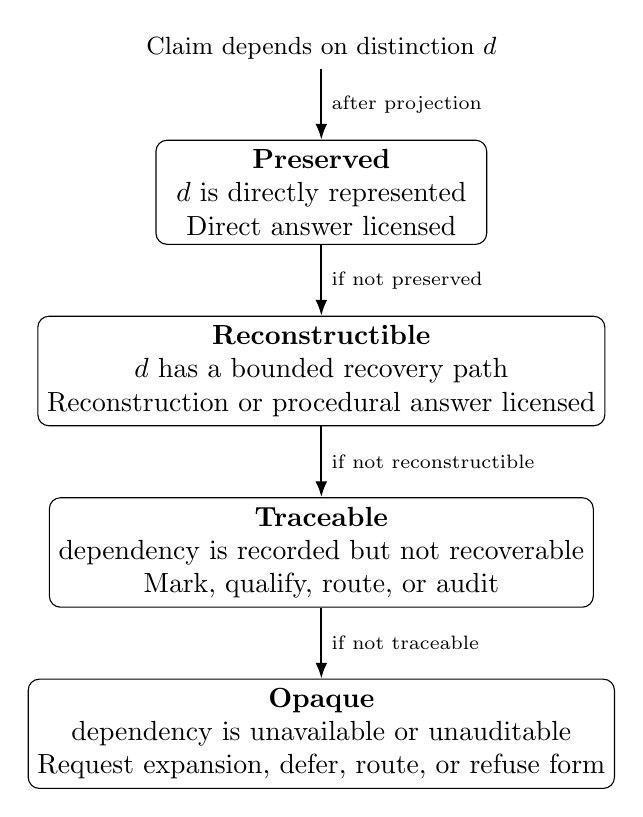
\begin{tikzpicture}[
    node distance=0.9cm,
    status/.style={
        draw,
        rounded corners,
        align=center,
        minimum width=4.2cm,
        minimum height=0.8cm
    },
    question/.style={
        align=center,
        font=\small
    },
    arrow/.style={-{Latex[length=2mm]}, thick}
]

\node[question] (claim) {Claim depends on distinction $d$};
\node[status, below=of claim] (preserved) {\textbf{Preserved}\\$d$ is directly represented\\Direct answer licensed};
\node[status, below=of preserved] (reconstructible) {\textbf{Reconstructible}\\$d$ has a bounded recovery path\\Reconstruction or procedural answer licensed};
\node[status, below=of reconstructible] (traceable) {\textbf{Traceable}\\dependency is recorded but not recoverable\\Mark, qualify, route, or audit};
\node[status, below=of traceable] (opaque) {\textbf{Opaque}\\dependency is unavailable or unauditable\\Request expansion, defer, route, or refuse form};

\draw[arrow] (claim) -- node[right, font=\scriptsize] {after projection} (preserved);
\draw[arrow] (preserved) -- node[right, font=\scriptsize] {if not preserved} (reconstructible);
\draw[arrow] (reconstructible) -- node[right, font=\scriptsize] {if not reconstructible} (traceable);
\draw[arrow] (traceable) -- node[right, font=\scriptsize] {if not traceable} (opaque);

\end{tikzpicture}
\caption{Operational dependency-status pathway under projection. The diagram shows the response-governance cases used by the framework, not a claim that all epistemic support relations form a total order. As recoverability and auditability weaken, the strongest licensed answer form also weakens.}
\label{fig:dependency_status_ladder}
\end{figure}

Figure~\ref{fig:dependency_status_ladder} visualizes the operational pathway described in Table~\ref{tab:dependency_status_answer_forms}. It should be read as a decision sequence---directly available, otherwise boundedly recoverable, otherwise attributable without recovery, otherwise opaque---rather than as a claim that every possible support relation lies on one scalar epistemic axis.

\begin{table}[h]
\centering
\caption{Dependency status, representational support, and licensed answer forms.}
\label{tab:dependency_status_answer_forms}
\begin{tabular}{lll}
\toprule
\textbf{Status} & \textbf{Support in representation} & \textbf{Licensed answer forms} \\
\midrule
Preserved & Distinction directly represented & Direct answer, ordinary correction \\
Reconstructible & Bounded recovery path available & Reconstruction, procedural answer \\
Traceable & Dependency recorded but not recoverable & Mark, qualify, route, audit \\
Opaque & Dependency unavailable or unauditable & Request expansion, route, defer, or refuse form \\
\bottomrule
\end{tabular}
\end{table}

The key boundary is between recovery and attribution. A traceable dependency preserves an accountable relation to the missing support without preserving enough information to recover the query-relevant distinction itself.

The boundary between reconstructible and traceable depends on whether the representation contains enough information to recover the distinction needed by the query, not merely enough information to identify where that distinction once came from. For example, a source hash, citation identifier, or provenance pointer may make a dependency traceable by recording that a claim depends on an external source. It is reconstructible only if the representation available to the reasoner also includes, retrieves, or otherwise supplies enough source content and recovery rules to determine the query-relevant distinction. If the pointer records that support exists but the relevant content is unavailable, the dependency is traceable rather than reconstructible. If even the dependency or source relation is not represented, the status is opaque.

This distinction is central for retrieval-augmented and tool-using AI systems. A retrieved document identifier, citation, tool-call trace, or audit log may make a dependency traceable without making the claim reconstructible. If the system cannot access the relevant source content, execution state, or recovery rule, then it should not treat the pointer as support for the claim. In safety and security settings, confusing traceability with reconstructability can produce false assurance: the system appears grounded because it has a pointer, but the representation available to the reasoner does not actually support the conclusion.

This ladder separates existence from operational support. Identifiability is an existence condition: if $q$ is identifiable under $P$, then some function from $R$ to the answer exists. Reconstructability is an operational condition: the system has an explicit recovery path, rule, derivation, proof, provenance structure, or bounded procedure that licenses the answer from the representation it actually uses. A query may be identifiable in principle while not being reconstructible for a particular system if the relevant recovery path is unavailable to that system.

Preserved and reconstructible distinctions can support inference. Traceable distinctions support accountability for transformation or loss, but not recovery of the original relation. Opaque loss supports neither inference nor audit. This ladder is therefore not a complete theory of provenance or explanation; it specifies what kind of support a downstream claim has after projection.

Dependency status, relative to the dependencies currently recognized as material, is the structural relation that later requirements are designed to preserve across reasoning steps, representation changes, correction attempts, and answer-form selection. Observability makes possible the detection or marking of unsupported dependency status. Bounded correction prevents a system from changing dependency status silently during repair. Non-collapse prevents claims supported at one level, such as a representation, intermediate state, or selected explanation, from being treated as if they were supported at another. The requirements that follow should therefore be read not as independent virtues, but as constraints on preserving dependency status under reasoning. When reasoning discovers a new dependency or a new relation among existing objects, the relevant invariant is not preservation of the earlier graph unchanged. It is preservation of the newly discovered constraint and its effect on subsequent licensing.

Real systems may attach qualifiers such as probabilistic, partial, prior-dependent, or provenance-conflicted to these base statuses. Such qualifiers refine the operational partition rather than converting it into a total ordering.

\section{Admissibility as Structural Licensing Under Projection}

In this framework, admissibility is a licensing relation among dependency status, operational validity, and response form. A direct claim is licensed only when the operative representation preserves or boundedly reconstructs the distinctions required to support it. A proposed action or continuation is additionally licensed only when it satisfies, or admits bounded return to, the operational validity conditions of the declared regime. When required distinctions are merely traceable or detectably unavailable, only weaker forms---such as qualification, conditionalization, routing, representation expansion, or refusal of the requested form---remain admissible. The requirements in this section are introduced as conceptual design constraints. Here, the goal is to show why these requirements naturally arise from the dependency-status problem.

The formal result above does not by itself specify a complete reasoning policy. It specifies a dependency problem: after projection, a claim may be supported by distinctions that are preserved, reconstructible, merely traceable, or opaque. A structurally reliable reasoning process must therefore avoid treating these dependency statuses as interchangeable.

These requirements are privileged only in a limited sense: they correspond to three generic ways that dependency status can be misrepresented after projection. First, the status of a dependency may fail to become visible at all; this motivates observability of loss-relevant state. Second, the system may silently strengthen the status of a dependency during repair, treating traceable or opaque loss as if it had become reconstructible; this motivates bounded correction. Third, the system may transfer dependency status across representational levels, treating support for a representation, proxy, intermediate state, provenance pointer, metric, or selected explanation as support for the underlying system or final claim; this motivates non-collapse of distinct levels.

Other mechanisms, such as calibration, provenance preservation, abstraction refinement, uncertainty representation, and compositional consistency, remain important. On this account, they are not rivals to the three requirements. They are implementation mechanisms, refinements, or domain-specific specializations. The three requirements are singled out because each blocks a distinct generic route by which unsupported dependency status can be promoted into apparently supported inference. The three requirements below should therefore be read as failure-preserving constraints rather than as a complete theory of reliable reasoning.

We describe the three requirements in turn.

\subsection{Partial Observability of Loss-Relevant State}

Observability of loss is necessarily partial and relative. A reasoning system need not be able to detect every distinction collapsed by projection; in general, it cannot. The requirement is not complete detection of loss, but preservation of detectable loss conditions relative to the representational language, metadata, or meta-representation available to the system. This includes:

\begin{itemize}[leftmargin=1.5em]
    \item ambiguity between multiple consistent interpretations,
    \item absence of necessary variables or context,
    \item dependence on assumptions not encoded in the representation.
\end{itemize}

In the formal terms above, partial observability means that the system can sometimes detect evidence that the requested query $q$ may not be constant over the equivalence class induced by $P$, relative to the distinctions it can express. When such evidence is available, the system must preserve it rather than treating the query as resolved.

Without observability, the system cannot distinguish between an identifiable query with a known answer and a non-identifiable query that only appears determinate after projection.

If such conditions are not observable within the system, they are effectively treated as resolved, even when they are not. This leads to outputs that appear complete but are based on unacknowledged gaps.

Observability does not require recovery of the missing information. In information-theoretic terms, it requires preserving enough side information about the projection, metadata, provenance, missing variables, ambiguity, or unsupported assumptions to represent detectable insufficiency as insufficiency. Failure of observability produces hidden loss: the system proceeds as if all relevant distinctions were present even when the representation no longer supports them.

\subsection{Bounded Correction}

Correction is bounded relative to a projection $P:S\rightarrow R$ when it can revise an incorrect result using only distinctions encoded in the representational state $R$. Here $R$ includes not only object-level data, but any explicitly represented metadata, provenance information, uncertainty markers, priors, task constraints, or assumptions available to the reasoning process. If correction requires distinguishing between states that are equivalent under $P$ and not distinguished anywhere in $R$, then the problem is not ordinary error correction within the representation. It requires representation expansion, new information, or an explicit assumption that changes the representational state.

While bounded correction concerns preserving the information basis during revision, non-collapse concerns preserving the role distinctions among representational objects. A system may satisfy bounded correction yet still collapse levels by treating a representation as equivalent to the system it represents, or by treating a selected explanation as uniquely determined by the available evidence.

The important point is not that correction must be small in a purely computational sense. It is bounded when the correction is licensed by distinctions already encoded in $R$, or by an explicit refinement that produces a new representation $R'$. A correction that silently imports distinctions not encoded in $R$ is not correction within $R$; it is an unmarked transition to a different representational state. For example, recomputing a formula from the same represented table is bounded correction; inventing a missing variable needed by the formula is not.

It is useful to distinguish two cases. In correction within $R$, the query is identifiable under the current representation and the system revises an incorrect answer using distinctions already available in $R$. In correction by refinement, the system explicitly moves from $R$ to a richer or different representation $R'$ by obtaining new information, adding a stated assumption, retrieving a source, or exposing metadata that was not previously represented. The second case may be admissible, but it is not correction within the original representation. It is bounded only if the transition from $R$ to $R'$ is explicit and the new information basis is marked. Thus bounded correction does not mean that a representation can never change. It means that correction must not silently change the information basis of the representation while presenting the result as if it followed from the original $R$.

A related consequence applies when reasoning under unresolved representational uncertainty must guide intervention rather than merely revise a claim. Bounded correction does not itself determine which action should be preferred, since action selection may depend on utilities, policies, authority, and other decision commitments not supplied by the represented evidence. It does, however, expose a structural difference among otherwise admissible actions. When the current representation leaves loss-relevant distinctions unresolved, an action that preserves observability, reversibility, and a bounded path for subsequent correction retains capabilities that an irreversible intervention may destroy. Thus uncertainty about the adequacy of the current representation can support a preference, under an explicitly declared decision rule, for interventions whose consequences remain detectable, attributable, and boundedly revisable. This is an interventional consequence of bounded correction rather than an extension of evidential support: it constrains how strongly a system commits under unresolved loss without determining the substantive value or policy according to which the action is selected~\cite{Fist2026}.

Without bounded correction, a system may appear to repair an error while actually importing information not present in the representation, thereby simulating access to the original state space $S$.

This requirement separates valid correction from implicit reconstruction. If correcting a result requires unsupported new assumptions, wholesale replacement of the representation, or unbounded reconstruction of the problem state, then the issue is no longer ordinary error correction. It is either representational loss or a representation failure.

Bounded correction ensures that:

\begin{itemize}[leftmargin=1.5em]
    \item errors can be repaired without silently changing the information basis of the representation,
    \item the distinction between error and loss is preserved in practice,
    \item correction remains a property of the reasoning process rather than an artifact of external intervention.
\end{itemize}

Failure of bounded correction leads to systems that appear to improve through repeated revision, but in fact introduce new assumptions or hidden state at each step.

\subsection{Non-Collapse of Distinct Levels}

A reasoning system must preserve role distinctions between objects that occupy different positions in the reasoning process. In dependency-status terms, non-collapse requires that support not be transferred across representational levels unless the dependency licensing that transfer is itself preserved, boundedly reconstructible, or explicitly conditioned. A representation may support a claim about the representation without supporting the same claim about the underlying system. A proxy may support a claim about the proxy without supporting the same claim about the target. A selected explanation may be consistent with the represented evidence without being uniquely licensed by it.

The relevant invariant is therefore not that all levels have the same structure, but that dependency status must not be silently promoted across levels. A preserved dependency at one level must not be treated as preserved at another level unless the relation between those levels is also preserved or reconstructible. Likewise, a traceable or opaque dependency must not become apparently reconstructed merely because it is attached to a fluent explanation, a metric, a provenance pointer, a selected model, or an aggregate representation.

This can be understood as a requirement of \emph{typed support preservation}. Support is attached not only to a proposition, but to a relation between a particular reasoning object or level and the dependency that licenses a claim about it. A transfer of support from one object to another therefore requires a represented transfer condition.

Schematically,

\[
\operatorname{Supp}(x,d)
\not\Rightarrow
\operatorname{Supp}(y,d)
\]

unless the relation carrying support from \(x\) to \(y\) is itself preserved, boundedly reconstructible, or explicitly conditioned. Non-collapse therefore prohibits \emph{unlicensed support transfer}: a representation cannot inherit the epistemic status of the world, a proxy that of its target, a provenance pointer that of source content, or a local judgment that of a composed system merely because the two objects are operationally connected.

In particular, the system must not collapse:
\begin{itemize}[leftmargin=1.5em]
    \item a representation with the underlying system it represents,
    \item a proxy or metric with the target property it measures,
    \item a provenance pointer with recoverable source support,
    \item provenance that a source participated in a determination with permission for that source to determine the target in the role it played,
    \item an intermediate reasoning state with a final conclusion,
    \item a selected explanation with the full set of explanations consistent with the representation,
    \item persistence of a reasoning operation with preservation of the conditions that license its use,
    \item a local component-level judgment with a claim about the composed system.
\end{itemize}

In particular, provenance and permission should not be collapsed. A representation may preserve which source, rule, or commitment participated in selecting an outcome while failing to preserve whether that determinant was licensed to play that role. The result may therefore remain traceable without remaining sufficient for the governance judgment that depends on the missing source--target--role relation.

The same distinction applies to reusable reasoning operations. A representation may preserve enough structure to execute a heuristic, procedure, scaffold, or transformation without preserving the context in which that operation was originally justified. Executability is therefore a property of the represented operator, while applicability is a dependency claim about the relation between that operator and the present state. Collapsing these levels allows a successfully preserved method to acquire unwarranted authority merely because it remains usable.

In each case, the collapse has the same form: a projected object inherits a stronger dependency status than the representation licenses. A representation is treated as the world, a proxy as the target, a pointer as source support, a partial reasoning state as a conclusion, a selected explanation as uniquely determined, or a local component judgment as a composed-system judgment. This makes projection loss invisible because the system can no longer track which dependency status belongs to which level.

These distinctions may coincide in specific cases, but they are not equivalent in general. Collapsing them prematurely removes the ability to track where information originates and how conclusions are derived.

For example, treating a selected explanation as if it were uniquely determined by the data conflates the space of possible models with the subset supported by the representation. Similarly, reducing a multi-dimensional decision to a single value collapses distinct evaluative dimensions into a single outcome.

Failure of level separation results in premature convergence, where the system commits to a single interpretation without preserving alternative possibilities that remain consistent with the available information.

\subsection{Structural Role of the Requirements}

Together, these requirements preserve the distinction between what is known, what can be corrected, and what has been lost. A system that satisfies them does not eliminate failure; it keeps failures detectable and keeps reasoning grounded in the structure of the representation. When they are absent, outputs may appear coherent while the reasoning process has diverged from the information available to it.

\section{Behavioral Consequences: Matching Answer Form to Dependency Status}

Because admissibility licenses response form, dependency status determines what claims may be presented as supported, while operational validity determines what actions or continuations may proceed. A direct answer is licensed only when the required dependency is preserved or boundedly reconstructible. An associated action must also be operationally valid or boundedly restorable within the declared regime. When either condition fails, the response must condition, weaken, reframe, ask, trace, route, constrain, or decline rather than preserve the appearance of determinacy or permission.

Respecting these constraints does not make reasoning systems infallible. It changes the status of their failures. Unsupported claims become visible rather than hidden; ambiguity is represented rather than suppressed; correction remains tied to the information basis of the representation; and decisions under non-identifiability are marked as decisions rather than inferred conclusions.

For AI reasoning systems, especially safety-critical ones, this changes what counts as a reliable answer. A reliable system should not merely be fluent, decisive, or consistent with a preferred output format. It should calibrate the form of its answer to the dependency status of the claim: direct when support is preserved, procedural when support is reconstructible, conditional when assumptions are required, trace-marked when support is external, and blocked or rerouted when the dependency is opaque.

\section{Diagnostic Examples}

These cases are not intended to estimate the frequency of projection-induced failures. They are diagnostic probes showing how the framework distinguishes unsupported determinacy, admissible conditional action, ordinary error, excessive abstention, and ambiguous dependency-status classification.

\subsection{Case 1: Scalarization and Proxy Collapse}

In this scenario, the system is required to produce an approval decision using a single numeric metric with no caveats. This constraint forces multiple dimensions of risk into a single value, creating the familiar possibility that optimization or decision-making over a proxy ceases to preserve the distinctions that matter to the underlying objective~\cite{Goodhart1975}. The relevant query is not merely ``which option maximizes the metric?'' but ``which decision is justified given reversibility, uncertainty, causal structure, and decision criteria?'' If two underlying states map to the same scalar value while requiring different decisions along one of these dimensions, then the decision query is not identifiable under the scalar projection.

A structurally reliable response should identify the scalar projection as insufficient for the decision query. The result need not be refusal. The system may request a richer representation, branch over unresolved risk dimensions, or make an explicitly labeled policy decision under non-identifiability. The inadmissible move is to present the scalarized answer as an inference justified by the metric alone.

\subsection{Case 2: Responsibility Assignment Under Causal Collapse}

In this scenario, the system is asked to assign responsibility for a failure to a single individual, despite the presence of multiple interacting causes. The relevant query is not simply ``who can be named as responsible?'' but ``which causal structure best explains the failure?'' If distinct causal structures map to the same single-person attribution, then responsibility is not identifiable under that projection.

A structurally reliable response should avoid treating one selected actor as if that actor were uniquely determined by the representation. It may instead separate individual action, process failure, system-level interaction, and unresolved evidence. The point is not to avoid responsibility claims altogether, but to preserve the dependency status of the attribution being made.

\subsection{Case 3: Traceability Without Source Reconstruction}

A common language-model failure occurs when a system is asked to summarize or cite information that is not present in its context. The projected representation contains topic cues, stylistic patterns, and plausible associations, but it does not contain the source-level distinction between what was actually observed and what is merely likely.

The relevant query is not simply ``what answer is plausible?'' but ``which claims are supported by the provided source?'' If two underlying states map to the same representation---one in which a claim is source-supported and one in which it is merely plausible---then source support is not identifiable under the projection. A structurally reliable response should separate supported claims from plausible but unsupported claims, request the missing source, or decline to assert source support.

\subsection{Case 4: Decision Under Non-Identifiability}

Not every non-identifiable query requires inaction. Suppose a triage system must choose between two actions under time pressure, but the representation does not contain enough information to determine which action is uniquely optimal. Two underlying states may map to the same representation while requiring different optimal actions under full information.

In this case, the query ``which action is uniquely best?'' is not identifiable under the projection. However, a decision may still be justified by an explicit rule, such as minimizing worst-case harm, deferring actions that would commit the system to loss beyond bounded correction, or selecting the option with a bounded fallback path. The decision is admissible only if it is marked as a policy choice under non-identifiability rather than as an inference uniquely determined by the representation.

The chosen policy must also satisfy the operational conditions of the declared regime. Marking an action as a decision rule resolves the inference-status problem, but it does not by itself establish that the action is authorized, reversible, feasible, or otherwise operationally valid.

\subsection{Case 5: Ambiguous Dependency Status Under Limited Observability}

Some cases cannot be cleanly classified from the current representation alone. Suppose a system gives an unsupported causal explanation, but the representation does not show whether the explanation came from hidden evidence, a valid prior, or an invented assumption. From the output alone, the failure may look like representational loss, ordinary error, or unjustified decision under uncertainty.

In this case, the framework does not by itself determine the correct classification. It identifies what must be made observable: whether the explanation is supported by information in the representation, by an explicit prior or decision rule, or by an unsupported assumption. This limit case is important because the framework does not eliminate projection; it specifies what additional structure must be exposed for classification to be reliable.

\subsection{Summary of Behavioral Modes}

The examples distinguish restructuring, conditional decision, representation expansion, trace marking, and refusal of the requested answer form as possible responses to non-identifiability. They also show that the framework should not be used as a blanket abstention policy: when a query is identifiable under the current representation, ordinary correction remains appropriate. The central requirement is not caution for its own sake, but matching the answer form to the dependency status of the claim.

\section{Applications}

Dependency status can be used as a design and evaluation lens for several AI reasoning, safety, and security problems.

\paragraph{Security copilots, code assistants, and incident response.}
Security and incident-response assistants often reason from compressed code context, alert summaries, deployment traces, and partial telemetry. The framework requires such systems to distinguish vulnerabilities or root causes supported by represented evidence from recommendations that depend on missing code paths, runtime configuration, threat models, event ordering, or logging conditions. When these distinctions are absent or only traceable, the system should mark the missing dependency, propose discriminating tests, request representation expansion, or offer bounded mitigations rather than present a single unsupported cause or fix as determined.

\paragraph{Retrieval-augmented generation and source grounding.}
RAG systems frequently expose provenance pointers, citations, or retrieved snippets. The dependency-status ladder distinguishes traceability from reconstructability: a pointer records a dependency, but only available source content and recovery rules can support the claim. This provides a concrete audit target for hallucination and false-grounding failures.

\paragraph{Agentic systems.}
Agents act from compressed internal state: task instructions, memory, tool outputs, environmental observations, and inferred user intent. Before acting, an agent should determine whether the distinctions required for action are preserved or reconstructible: authorization, reversibility, environmental state, user intent, and safety constraints. When these distinctions are opaque, the agent should request representation expansion, route to a human or tool, or act only under an explicit bounded policy.

\paragraph{User modeling and Theory-of-Mind-like behavior.}
Dependency status also applies to AI systems that model users or other agents. A system often infers what a user knows, wants, intends, believes, or cannot distinguish from partial interaction traces. These inferences are projection-sensitive: observed behavior may preserve some distinctions while leaving others merely plausible, traceable to prior context, or opaque. A safety-relevant user model should therefore mark whether claims about another agent's state are directly observed, reconstructible from interaction, dependent on an explicit assumption, or unsupported. This does not require treating the AI system as having humanlike inner experience. It treats Theory-of-Mind-like behavior as reasoning under projection over another agent's representation.

\paragraph{Reasoning scaffolds, procedures, and inherited decision rules.}
Reusable reasoning procedures are themselves subject to projection. A prompt scaffold, diagnostic checklist, review procedure, policy rule, or institutional heuristic may remain available long after some of the assumptions or contextual distinctions that originally governed its use have disappeared from the operative representation. A system should therefore distinguish whether it can execute a procedure from whether the dependencies licensing that procedure remain preserved or reconstructible in the current case. Successful execution does not by itself establish appropriate application.

\paragraph{Evaluation and benchmark design.}
Standard evaluation may reward correct-looking answers even when the representation does not support them. Projection-aware evaluation should test whether systems change behavior when observability changes: refusing unsupported determinacy at low observability, ranking hypotheses under partial evidence, and becoming appropriately decisive when the relevant distinction becomes observable. This makes dependency status a measurable target rather than a purely philosophical concern.

\section{Why Existing Methods Can Miss This Failure}

Existing methods can improve performance within a representation without testing whether the representation preserves the distinctions required by the query. Optimization can improve a proxy while hiding loss of task-relevant structure. Prompting can make reasoning more detailed without verifying that the needed dependency is represented. Evaluation can reward a plausible answer while failing to test whether a determinate answer was identifiable from the available evidence.

The common mismatch is that these methods often operate over $R$, while the failure arises from the projection $P:S\rightarrow R$. A source-grounding benchmark may check whether an answer contains a citation, but not whether the cited content preserves the distinction needed by the claim. An incident-response benchmark may reward naming a plausible cause, while failing to penalize the system for ignoring that telemetry cannot distinguish among several causes.

This does not mean optimization, prompting, or evaluation are misguided. It means they require an additional structural check: whether the claim's dependency status is preserved, reconstructible, traceable, or opaque under the representation being used, and whether a proposed continuation satisfies or admits bounded return to the operational validity conditions of the declared regime.

\section{Relation to Existing Frameworks}

The argument in this paper overlaps with several established lines of work. In statistics and causal inference, identifiability asks whether a target quantity can be determined from the available observational structure~\cite{Pearl2009}. In statistical decision theory, comparison of experiments and sufficiency ask when one signal or observation preserves enough information for a class of decisions~\cite{Blackwell1953}. In partially observable decision processes, agents must act over incomplete state representations~\cite{Kaelbling1998}. Work on state abstraction evaluates compressed states according to whether they preserve value-, policy-, reward-, transition-, or model-relevant properties~\cite{Li2006}. In formal methods and abstract interpretation, abstraction maps concrete states into reduced domains while preserving selected properties~\cite{CousotCousot1977}; counterexample-guided abstraction refinement studies how an abstraction may be refined when it is too coarse for the property being checked~\cite{Clarke2000CEGAR}. In information-theoretic approaches such as the information bottleneck, compressed representations are evaluated by the task-relevant information they retain~\cite{Tishby1999}.

A particularly close neighboring framework is partial identification, which studies what can be learned when available observations and maintained assumptions identify a set of possible values rather than a unique value~\cite{Manski2003,Manski2008}. The present account shares partial identification's refusal to treat observational equivalence as point determination. Its additional concern is operational: dependency status distinguishes whether a query-relevant distinction is directly preserved, boundedly reconstructible, merely traceable, or opaque, and uses that status to constrain the form in which a reasoning system may answer. Partial-identification bounds characterize the set of values compatible with an information structure and maintained assumptions; the dependency-status framework additionally records what kind of support or recovery path licenses a response and how the system should behave when such support is unavailable.

The framework also overlaps with selective prediction, abstention, conformal prediction, and hallucination detection. Selective classification and reject-option methods study when a predictor should abstain rather than answer, often by optimizing a risk--coverage tradeoff~\cite{GeifmanElYaniv2017,GeifmanElYaniv2019}. Conformal prediction provides calibrated prediction sets or uncertainty guarantees under distributional assumptions such as exchangeability~\cite{Vovk2005,Shafer2008}. Work on hallucination in natural-language generation and large language models studies unsupported or fabricated generated content, including methods for detecting inconsistency or unsupported factual claims~\cite{Ji2023,Manakul2023}. The present framework is complementary to these literatures: it focuses on whether the operative representation preserves the distinction required by the requested claim and, therefore, whether the answer form is licensed by dependency status rather than confidence alone.

Across these traditions, the closest point of contact is the treatment of projection failure as a failure of query-relative sufficiency. The additional step taken here is to treat the surviving relation between a claim and its information basis as typed dependency status, to use that status to govern response form, and to distinguish the status that actually obtains from the status a bounded reasoner assesses and reports.

Recent structural accounts sharpen this boundary further. Bruhacs develops task-relative sufficiency in terms of the invariants, selectors, and operators that must survive projection, together with minimal-support results identifying least representations sufficient for specified epistemic tasks~\cite{Bruhacs2026Projection,Bruhacs2026Hidden}. His subsequent analysis of AI inference also establishes limits on task-blind reconstruction and purely public selection across heterogeneous targets~\cite{Bruhacs2026Limits}. These results provide a useful exact baseline for the present account: for a specified query, one may ask what minimal structure must survive for exact determination to remain possible. The framework developed here is primarily concerned with the bounded-reasoner regime in which the operative representation does not meet that baseline, the reasoner cannot establish that it does, or operational validity imposes an additional constraint beyond informational sufficiency. Its question is therefore not only what representation would be sufficient in principle, but what claim or continuation remains licensed when sufficient structure is absent, uncertain, trace-only, or boundedly recoverable.

A complementary line of work by Swanson distinguishes loss introduced when a target is stabilized from loss introduced when that target is subsequently rendered, and separates boundary overextension from representational overextension~\cite{Swanson2026Monist}. His carrier framework further characterizes best-achievable task loss under bounded representation and the improvement of adequacy under representational refinement~\cite{Swanson2026Carriers}. These distinctions are compatible with the \(F\xrightarrow{B_{\Gamma}}S_{\Gamma}\xrightarrow{P_{\Gamma}}R\) extension used here. The present account uses those neighboring results as structural inputs to a different operational question: how dependency recoverability and auditability, answer form, operational permission, and actual--assessed--reported status should remain distinguished for a bounded reasoner. These differences are complementary rather than competitive: exact sufficiency characterizes what would need to survive; representation-risk analysis characterizes consequences of what does not; admissibility governs what a bounded reasoner may claim or do given the structure that remains.

This distinction is especially important for partial-observation models. Partial-observation methods, including POMDP-style accounts, can represent uncertainty over hidden states and help identify ambiguity, underspecification, or missing evidence. Hidden state, however, is not identical to projected-away structure. A distinction may be unavailable from the current representation rather than merely unknown within it. Detecting hiddenness can indicate that the representation is incomplete; reconstructibility governance determines whether the claim remains admissible, must be weakened, requires representation expansion, can be traced, or should be blocked.

This paper does not claim that these frameworks are equivalent, nor does it replace their domain-specific accounts of identifiability, abstraction, observability, or belief-state update. Instead, it identifies a shared reasoning-system failure pattern: a downstream reasoner is asked to draw a determinate conclusion from a representation that may not preserve the distinctions required by the query. Prior work often specifies when a property is identifiable, when an abstraction is sound, when a statistic is sufficient, or when a belief state supports action. The failure analyzed here occurs when a reasoning system behaves as though the relevant identifiability, sufficiency, or preservation condition holds when it does not. Partial-observation methods are useful for representing hiddenness and maintaining uncertainty over modeled possibilities, but they do not by themselves establish that a query-relevant distinction survived projection or is boundedly reconstructible from the operative representation.

The error--loss distinction is consequently a diagnostic constraint on reasoning behavior. If the query is identifiable under the current representation and the system answers incorrectly, the failure is ordinary error. If the query is not identifiable, additional optimization, prompting, explanation, or evaluation within the same representation cannot by itself recover the missing distinction. The system must instead expand the representation, obtain new information, introduce an explicit assumption or decision rule, weaken the claim, or mark the dependency as traceable or opaque.

\section{Operational Implications}

A minimal implementation can treat admissibility assessment as a five-step diagnostic rather than as an oracle:

\begin{enumerate}
    \item Identify the claim, action, or continuation being licensed.
    \item Identify the distinctions on which that claim, action, or continuation depends.
    \item Check whether each distinction is preserved, reconstructible by a bounded procedure, merely traceable, or opaque in the operative representation.
    \item For a proposed action or continuation, check whether it satisfies or admits bounded return to the operational validity conditions of the declared regime.
    \item Select a response form jointly licensed by dependency status and operational validity: direct answer, bounded reconstruction, conditional answer, branch over assumptions, request for representation expansion, trace marking, routing, constraining, deferral, or refusal of the requested form.
\end{enumerate}

The diagnostic also requires a distinction between actual, assessed, and reported dependency status. For operative representation \(R\), let
\[
\delta^{*}_{\Gamma,q,R}(d)
\]
denote the status that dependency \(d\) actually has relative to query \(q\) and operative regime \(\Gamma\);
\[
\widehat{\delta}_{\Gamma,q,R}(d)
\]
the status assessed by the reasoner; and
\[
\widetilde{\delta}_{\Gamma,q,R}(d)
\]
the status reported in the resulting answer or reasoning artifact. The normative framework constrains response form relative to actual dependency status, while practical systems can act only through imperfect assessments. Evaluation must therefore consider both whether the assessed status is accurate and whether the reported answer form faithfully reflects that assessment.

These three quantities should not be identified. In particular,

\[
\widehat{\delta}_{\Gamma,q,R}(d)
\neq
\delta^{*}_{\Gamma,q,R}(d)
\]

is possible even when the reasoner follows its assessment procedure correctly. The operative representation may itself omit the evidence needed to determine whether a dependency is preserved, reconstructible, traceable, or opaque. A bounded reasoner can therefore be locally correct relative to its represented evidence while being mistaken about the adequacy of that evidence. Neighboring impossibility results reinforce the general concern: Bruhacs shows that the observational or public representation alone does not in general determine the appropriate hidden reconstruction across heterogeneous tasks~\cite{Bruhacs2026Limits}. The distinction introduced here is different: it asks how that underdetermination affects a reasoner's assessment and report of its own dependency status.

This creates a second-order admissibility problem. First-order admissibility asks whether the answer form is licensed by the actual dependency status. Second-order admissibility asks what the reasoner is licensed to claim about its own assessment of that status. Successful execution of an admissibility procedure does not certify that the representation supplied enough structure for the procedure to classify its own applicability correctly.

The reported status introduces a further requirement:

\[
\widetilde{\delta}_{\Gamma,q,R}(d)
\preceq
\widehat{\delta}_{\Gamma,q,R}(d),
\]

where \(\preceq\) means ``no stronger than'' in the dependency-status ordering, subject to any qualifiers attached to the assessment. A system should not report stronger support than it assessed. But satisfying this reporting constraint does not establish that the assessment itself was correct:

\[
\widetilde{\delta}
\preceq
\widehat{\delta}
\quad\not\Rightarrow\quad
\widehat{\delta}=\delta^{*}.
\]

The distinction therefore separates two failure modes. \emph{Assessment error} occurs when the reasoner misclassifies actual dependency status. \emph{Reporting inflation} occurs when the answer presents a stronger dependency status than the reasoner's own assessment supports. Runtime governance can directly constrain the second failure; the first remains subject to the same projection limits that motivate the framework as a whole.

The purpose of this section is not to define the full protocol, evaluation framework, or control layer. The goal here is only to show how the dependency-status ladder naturally yields operational targets: answer-form governance, evaluation under projection stress, interface-level representation repair, and audit fields for downstream systems.

When assessed status is uncertain, the system should preserve that uncertainty in the reported status rather than silently promote the claim. This requirement is analogous to Swanson's \emph{non-laundering} condition for typed institutional reason-giving, under which reported grounds should track the grounds that actually did the decisional work~\cite{Swanson2026Typed}. In the present setting, uncertainty, assumptions, provenance limits, or unresolved dependencies that materially determine the reasoner's assessment should not disappear when the assessment is converted into a user-facing claim, action, or reasoning artifact.

\subsection{Evaluation by Structural Shape}

Evaluation can be organized around whether a response preserves the structural shape required by the query, rather than only whether it matches a domain-specific target answer. A responsibility query can be evaluated for preservation of individual, process, and system levels; a high-stakes decision for visibility of irreversible tradeoffs and residual risk; a source-grounded answer for separation between observed support and plausible reconstruction; and a compositional policy problem for revalidation under interaction or scale. Such diagnostics ask whether the answer has the right admissibility structure: what distinction is needed, whether it is preserved or reconstructible, whether loss is visible, and whether the system has confused inference with decision. These targets could be operationalized through controlled question sets that vary the represented distinctions, prompt constraints, and available recovery paths.

\subsection{Reasoning Scaffolds and Constraint Activation}

The same dependency-status distinctions can be used to constrain generation. A reasoning scaffold can require the system to preserve observability of loss-relevant state, avoid collapse of conceptual levels, keep correction bounded, distinguish error from loss, and revalidate conclusions under scale or composition. Such scaffolds do not prescribe a single reasoning style. They constrain which transformations are admissible when the system moves from a projected representation to an answer.

In addition, different tasks may require attention to different dependency-status risks. A source-grounding task may foreground observability and provenance; a responsibility-assignment task may foreground non-collapse of levels; a deployment decision may foreground bounded correction and scale revalidation. Task-specific activation of these dependency-status risks provides a control layer over reasoning without changing the underlying structural requirements.

\subsection{Interface and Question-Formation Uses}

Dependency-status distinctions can also be used before answer generation, as interaction lenses for forming better questions. A user interface need not treat the query as fixed. It can help users select objects, group them, specify relations, and choose a reasoning lens such as observability, reconstructability, traceability, admissibility, scale, or non-collapse. The resulting query is then not merely a request for an answer, but an explicit statement of which distinctions must be preserved during reasoning.

On this view, question formation is itself a projection-management task. The user and system jointly determine which distinctions matter before inference proceeds. This is especially important in settings where the initial question collapses roles, scales, sources, or decision criteria that must remain separate for the answer to be admissible.

In interactive systems, clarifying questions are one mechanism for representation repair. A clarification request is not merely conversational hesitation or a user-interface convenience. It is a way of enriching, refining, or changing the projection so that the requested query becomes identifiable, boundedly reconstructible, or explicitly conditional. Conversely, if the missing distinction does not affect the dependency status of the requested claim, the system should not treat clarification as required. The point is not to ask more questions, but to ask when the current representation does not support the requested answer form.

\subsection{Audit and Dependency Status}

Finally, the dependency-status ladder suggests audit fields for downstream systems. A claim can be marked according to whether its required dependency is preserved, reconstructible, traceable, or opaque. Such markings do not guarantee correctness, but they make visible whether a conclusion is supported by the representation, recovered through an explicit path, dependent on a recorded but unrecoverable relation, or unsupported by observable provenance.

This allows downstream users or systems to distinguish claims that are inferentially supported from claims that are merely decisions, assumptions, or unresolved dependencies under non-identifiability.

Taken together, these uses show how dependency status can guide downstream scaffolds, evaluation harnesses, runtime systems, interfaces, and audit mechanisms without requiring a single domain-specific answer metric.

\section{Scope and Limits}

This paper describes structural conditions for reasoning under projection. It does not attempt to provide a complete theory of reasoning, nor does it claim to resolve all sources of uncertainty or failure. This section clarifies the scope of the claims and the limits of what these constraints guarantee.

\subsection{What This Does Not Solve}

Respecting the constraints described in this paper does not eliminate the fundamental challenges associated with reasoning over incomplete or compressed representations.

In particular, it does not:

\begin{itemize}[leftmargin=1.5em]
    \item guarantee that a system will produce correct conclusions,
    \item eliminate ambiguity in cases where multiple interpretations remain consistent,
    \item recover distinctions that are not preserved or boundedly recoverable under the current representation,
    \item ensure that all relevant variables are present in the representation,
    \item prevent all forms of bias or misalignment in decision-making,
    \item guarantee that the system has discovered every dependency, stakeholder, constraint, alternative method, or intended use relevant to the query.
\end{itemize}

A fuller developmental account would need to explain how discovered constraints revise that structure and persist afterward; the present framework does not claim that such discovery can ever be complete.

\subsection{Dependence on Representation}

The behavior of a reasoning system under this framework depends on the representation over which it operates. Different representations preserve different distinctions, and therefore introduce different forms of loss.

Improving reasoning performance may require modifying the representation itself, not just the reasoning process applied to it. However, such changes alter the projection and therefore change the conditions under which reasoning operates.

This paper does not prescribe a single representation or assume that the operative representation remains fixed. It provides constraints that apply to a representation at a given stage of reasoning. A later stage may refine the projection, introduce a new distinction, attach a newly relevant constraint, or reformulate the query. Such revisions alter the state to which admissibility is applied and should therefore be explicit rather than silently attributed to the earlier representation.

\subsection{Diagnostic Pressure and Earned Observability}

The fact that a representation may omit a materially relevant distinction does not imply that every conceivable distinction should be represented in advance. Such a requirement would replace one failure mode with an unbounded demand for representational completeness, which the framework neither assumes nor requires. Instead, refinement can be driven by \emph{diagnostic pressure}: evidence that the current representation repeatedly prevents a materially relevant failure, disagreement, ambiguity, or unresolved alternative from being localized.

Diagnostic pressure may arise when independent reasoning processes diverge at an unresolved dependency, when repeated failures remain observationally indistinguishable, when an investigation repeatedly encounters inadequate provenance or logging, when correction requires information that the current representation consistently fails to preserve, or when an observed failure does not fit the distinctions supplied by the current model. The last case is especially important in adversarial and open-ended environments: the relevant failure class may not have been known when the representation was designed. Such evidence does not automatically identify a missing variable, dependency, or ontology, nor does it require permanent expansion of the modeled state. It establishes a narrower claim: the current representation is insufficient for diagnosing something that practical experience has shown to matter.

The resulting refinement should therefore be minimal and diagnostic where possible. A system may add telemetry, provenance, an explicit dependency relation, a discriminating test, a temporary probe, a retained distinction, or a richer representation. The aim is not to represent more state for its own sake, but to make a demonstrated class of failures more observable, attributable, or correctable. In this sense, additional structure \emph{earns} its place in the representation through demonstrated diagnostic value.

The same principle applies in reverse. Structure need not be retained merely because it was once represented. Dependencies that are redundant, cheaply reconstructible, no longer material to the governed query class, or costly to preserve relative to their diagnostic value may be compressed, summarized, or removed. Such dependency hygiene is compatible with structural reliability so long as the resulting representation does not silently claim support that depended on the discarded structure. The objective is sufficient diagnostic capacity, not maximal retention.

\subsection{Mechanism and Evaluation as Downstream Work}

The present paper specifies the structural failure mode rather than a complete implementation. A detector for representational loss would need to identify when a query depends on distinctions that are neither preserved, nor boundedly reconstructible, nor explicitly assumed in the current representation. A dependency-status implementation would need to represent whether a claim is preserved, reconstructible, traceable, or opaque.

Evaluation should therefore test not only whether a system reaches a target answer, but whether it changes behavior appropriately as the representation changes. One natural benchmark pattern is to compare compressed and enriched versions of the same task: when the compressed representation does not preserve the distinction required by the query, the system should avoid unsupported determinacy; when the enriched representation restores the distinction, the system should become correspondingly more decisive. This tests whether the system distinguishes representational loss from ordinary error rather than merely becoming more cautious.

\subsection{Empirical Vulnerability of the Practical Account}

The formal claims in this paper are conditional on their stated representational assumptions. In particular, the non-identifiability result follows when distinct states collapsed by the operative projection require different answers to the query. A separate empirical question is whether the dependency distinctions developed here provide useful explanations or predictions for actual reasoning systems. That broader practical claim should remain vulnerable to evidence rather than being inferred from the internal consistency of the formal account.

Evidence against the practical importance of the framework would include failure to observe meaningful behavioral differences between preserved, reconstructible, traceable, and opaque dependency conditions under independently designed evaluation; failure of controlled representation enrichment to produce the predicted change in licensed answer form; failure of relational or dependency structure to add diagnostic value beyond component-level information; or repeated external cases in which the framework's distinctions provide no useful explanatory or corrective advantage over simpler existing accounts. Such findings would not invalidate the elementary non-identifiability result itself, but they would weaken the claim that reconstructibility under projection identifies a practically important structure of AI reasoning failure.

\subsection{Self-Application Non-Certification}

The framework is itself subject to the conditions it describes. An admissibility procedure operates over a representation of the dependencies, regime, query, and available recovery paths. It therefore cannot infer from successful execution alone that those represented conditions were complete or adequate.

This yields a general principle:

\[
\boxed{
\text{successful execution of a reasoning or governance procedure}
\not\Rightarrow
\text{certification that its application was licensed}.
}
\]

Call this \emph{Self-Application Non-Certification}. The principle does not make admissibility assessment futile. It limits what such assessment certifies. A procedure may improve structural reliability, expose detectable loss, constrain reporting inflation, and require explicit recovery paths without becoming an oracle for the completeness of its own representation.

The practical consequence is that admissibility mechanisms should expose the basis and limits of their own assessments. They may classify represented dependencies, record unresolved conditions, request refinement, or qualify their own status judgments. They should not silently convert successful self-application into evidence that no relevant dependency was omitted upstream.

\subsection{Limits of Observability}

While the error--loss distinction requires observability of loss-relevant state, this observability is itself subject to projection. A system may be unable to represent certain forms of loss because the representation does not include the necessary structure.

This creates an important limitation: loss can only be detected relative to distinctions that the representation is capable of expressing. A system cannot observe every loss introduced by its own projection; it can only mark the boundaries where the current representation no longer supports a requested query.

In such cases, the system may be unable to indicate the specific lost distinction, even if loss exists. It may still be able to mark a weaker diagnostic condition, such as missing variables, unsupported assumptions, or insufficient provenance. This places a practical limit on how completely loss can be made visible within any given representation.

The practical target is therefore improved diagnostic visibility, not complete loss detection or representational completeness. The framework seeks to make consequential insufficiency increasingly observable where experience provides evidence that the current representation is inadequate, while retaining the recursive limitation that no represented diagnostic process can certify that every material dependency has been found.

\section{Conclusion}

AI systems reason from compressed representations: prompts, summaries, retrieved snippets, tool outputs, logs, metrics, memory, and policy artifacts. Compression is unavoidable, but it can collapse distinctions that later claims require. Some loss can arise even earlier, when the target state treated as relevant excludes a distinction needed by the eventual query; other loss arises when an adequate target is subsequently projected into an insufficient operative representation. When a query is not identifiable under the current representation, additional reasoning over that representation cannot recover the missing distinction. Put informationally, the missing distinction is not available for decoding from the current information basis.

The central error analyzed in this paper is misclassifying representational loss as recoverable inference error. This produces fluent but unsupported determinacy: hallucinated source support, overconfident root-cause attribution, unsafe action under missing state, or metric success that hides loss of relevant structure.

The proposed dependency-status taxonomy---preserved, reconstructible, traceable, and opaque---does not guarantee correctness and is not intended as a total ordering of epistemic states. It is an operational partition reflecting two separable questions: whether the required distinction remains directly available or boundedly recoverable, and whether an accountable dependency trail remains when recovery fails. Those statuses constrain answer form: direct when support is preserved, procedural when it is reconstructible, trace-marked or qualified when recovery fails but attribution remains, and blocked, expanded, or rerouted when the dependency is opaque.

The same discipline applies to the basis of support itself. Evidence, background assumptions or priors, and policy or decision commitments may all appear in the operative representation, but they do not perform the same epistemic role. A prior-supported preference should not be reported as evidence-determined, and a policy-selected action should not acquire evidential support merely because it is licensed to proceed. For actions and continuations, dependency support therefore remains distinct from operational permission and later selection. Where unresolved representational uncertainty remains, bounded correction nevertheless has an interventional consequence: among actions selected under an explicit policy or decision rule, preserving observability, reversibility, and bounded fallback capacity can preserve the possibility of later correction without pretending that the evidence itself selected the action.

The same separation applies to provenance of selection itself. Knowing which source or commitment determined an outcome does not by itself establish that the determinant was licensed to play that role; that licensing relation may itself be lost under projection even when the endpoint and its provenance survive.

Reasoning under projection is therefore not an edge case. It is the ordinary condition of AI systems operating over bounded context, retrieval, tools, summaries, metrics, memory, inherited procedures, and reusable reasoning scaffolds. The admissibility question is whether such systems can preserve the difference between what their representations determine, what they can reconstruct, what they can merely trace, and what they have lost, while also distinguishing informational support from operational permission to continue. In particular, preservation of a usable reasoning operation should not be mistaken for preservation of the contextual dependencies that license its application. Nor should successful execution of the admissibility framework itself be treated as certification that those dependencies were completely represented. The framework is recursively subject to projection: it can govern what is visible to it without guaranteeing that everything material has become visible.

Reliability under these conditions should therefore not be understood as approximation to an omniscient reasoner that represents every relevant fact, anticipates every failure class, and avoids every error. The more attainable structural objective is diagnostic legibility: when reasoning fails, disagrees, encounters unresolved ambiguity, or produces behavior that the current model cannot adequately classify, the representation should preserve enough structure to determine what can and cannot presently be localized, reconstructed, attributed, or corrected. Repeated inability to make such distinctions can itself become evidence that additional observability, a new dependency, or revision of the represented failure structure is warranted.

The framework developed here is necessarily relative to the dependency structure currently represented for the query. It can determine that a claim has stronger form than its represented support permits, but it does not assume that every relevant dependency was known when reasoning began. Practical progress may instead consist in discovering that the original question was misframed, that two concepts must remain separate, that a source dependency was hidden, that an action requires independent authority, or that a previously known concern constrains a new claim.

The resulting account is not a machine for producing final answers from fixed premises, nor a prescription to expand representations toward completeness. It is a framework for keeping the relationship among representations, dependencies, claims, actions, failures, and discovered constraints visible enough that later reasoning can diagnose where support became insufficient and refine the information basis when demonstrated need warrants doing so. The objective is not to prevent all error, but to prevent error from becoming unnecessarily opaque.

Future work should investigate the formal conditions under which these requirements are necessary or sufficient, how dependency status changes across successive projections, how projection-sensitive behavior can be evaluated, and how reasoning systems can implement admissibility checks without turning them into blanket abstention policies.

\begin{thebibliography}{99}

\bibitem{Amodei2016}
Dario Amodei et al.
\newblock Concrete Problems in AI Safety.
\newblock arXiv:1606.06565, 2016.

\bibitem{Blackwell1953}
David Blackwell.
\newblock Equivalent comparisons of experiments.
\newblock The Annals of Mathematical Statistics, 1953.

\bibitem{Bruhacs2026Hidden}
Lorand Bruhacs.
\newblock Hidden Structure and Explanation: Explanatory Descent and Minimal Hidden Support.
\newblock Preprint, 2026.
\newblock doi:10.5281/zenodo.19057860.

\bibitem{Bruhacs2026Limits}
Lorand Bruhacs.
\newblock The Limits of AI Inference: Abduction, Regularization and Non-Public Norm Selection.
\newblock Preprint, 2026.
\newblock doi:10.5281/zenodo.19411423.

\bibitem{Bruhacs2026Projection}
Lorand Bruhacs.
\newblock Task-Sufficient Inference and Explanation: Reasoning Under Projection.
\newblock Draft preprint, 2026.

\bibitem{Clarke2000CEGAR}
Edmund M. Clarke, Orna Grumberg, Somesh Jha, Yuan Lu, and Helmut Veith.
\newblock Counterexample-guided abstraction refinement.
\newblock CAV, 2000.

\bibitem{CousotCousot1977}
Patrick Cousot and Radhia Cousot.
\newblock Abstract interpretation: A unified lattice model for static analysis of programs by construction or approximation of fixpoints.
\newblock POPL, 1977.

\bibitem{Fist2026}
Tim Fist, Saif Khan, Tao Burga, Arthur Tellis, Ben Schifman, Jonah Weinbaum, and Olivia Scharfman.
\newblock How Should the US Prepare for Increasingly Automated AI R\&D? 23 Low-Regret Policy Recommendations.
\newblock Institute for Progress, August 6, 2026.

\bibitem{GeifmanElYaniv2017}
Yonatan Geifman and Ran El-Yaniv.
\newblock Selective Classification for Deep Neural Networks.
\newblock In \emph{Advances in Neural Information Processing Systems}, 2017.

\bibitem{GeifmanElYaniv2019}
Yonatan Geifman and Ran El-Yaniv.
\newblock SelectiveNet: A Deep Neural Network with an Integrated Reject Option.
\newblock In \emph{Proceedings of the 36th International Conference on Machine Learning}, 2019.

\bibitem{Goodhart1975}
Charles Goodhart.
\newblock Problems of Monetary Management: The U.K. Experience.
\newblock In \emph{Papers in Monetary Economics}, 1975.

\bibitem{Kaelbling1998}
Leslie Pack Kaelbling, Michael L. Littman, and Anthony R. Cassandra.
\newblock Planning and acting in partially observable stochastic domains.
\newblock Artificial Intelligence, 1998.

\bibitem{Li2006}
Lihong Li, Thomas J. Walsh, and Michael L. Littman.
\newblock Towards a unified theory of state abstraction for MDPs.
\newblock ISAIM, 2006.

\bibitem{Manakul2023}
Potsawee Manakul, Adian Liusie, and Mark J. F. Gales.
\newblock SelfCheckGPT: Zero-Resource Black-Box Hallucination Detection for Generative Large Language Models.
\newblock In \emph{Proceedings of EMNLP}, 2023.

\bibitem{Manski2003}
Charles F. Manski.
\newblock \emph{Partial Identification of Probability Distributions}.
\newblock Springer Series in Statistics. Springer, New York, 2003.

\bibitem{Manski2008}
Charles F. Manski.
\newblock \emph{Identification for Prediction and Decision}.
\newblock Harvard University Press, Cambridge, Massachusetts, 2008.

\bibitem{Pearl2009}
Judea Pearl.
\newblock Causality: Models, Reasoning, and Inference.
\newblock Cambridge University Press, 2009.

\bibitem{Savage1954}
Leonard J. Savage.
\newblock The Foundations of Statistics.
\newblock 1954.

\bibitem{Shafer2008}
Glenn Shafer and Vladimir Vovk.
\newblock A Tutorial on Conformal Prediction.
\newblock \emph{Journal of Machine Learning Research}, 9:371--421, 2008.

\bibitem{Shannon1948}
Claude Shannon.
\newblock A Mathematical Theory of Communication.
\newblock Bell System Technical Journal, 1948.

\bibitem{Swanson2026Carriers}
David T. Swanson.
\newblock Carriers and Adequacy for Purpose: A Formal Framework for Representation-Constrained Adequacy.
\newblock Manuscript, May 21, 2026.

\bibitem{Swanson2026Monist}
David T. Swanson.
\newblock Target Stabilization and Finite Representation: A Monist Framework.
\newblock Manuscript, May 21, 2026.

\bibitem{Swanson2026Typed}
David T. Swanson.
\newblock Typed Desk-Stage Editorial Triage: Discourse vs Dialectic Entry, Contribution Type, and Auditability.
\newblock Manuscript, 2026.

\bibitem{Tishby1999}
Naftali Tishby, Fernando C. Pereira, and William Bialek.
\newblock The information bottleneck method.
\newblock 1999.

\bibitem{Vovk2005}
Vladimir Vovk, Alex Gammerman, and Glenn Shafer.
\newblock Algorithmic Learning in a Random World.
\newblock Springer, 2005.

\bibitem{Ji2023}
Ziwei Ji, Nayeon Lee, Rita Frieske, Tiezheng Yu, Dan Su, Yan Xu, Etsuko Ishii, Yejin Bang, Andrea Madotto, and Pascale Fung.
\newblock Survey of Hallucination in Natural Language Generation.
\newblock \emph{ACM Computing Surveys}, 55(12), Article 248, 2023.

\end{thebibliography}
\end{document}

